\documentclass{beamer}
\usetheme{Madrid}

\usepackage{graphicx}
\usepackage{adjustbox}
\usepackage{tikz}
\usepackage{listings}

\usetikzlibrary{automata,arrows}
\pgfmathtruncatemacro\distance{1}

\lstset{language=erlang, basicstyle=\sffamily\footnotesize,
  keywordstyle=\color{blue}, numberstyle=\tiny, numbers=none,
  showspaces=false, showstringspaces=false, frame=tL,
  backgroundcolor=\color{black!5}, morekeywords={send, to, from} }

\title{Extracting Choreography Automata \\ for Program Understanding}
\author{Gabriele Genovese \\ Supervisor: Prof. Cinzia Di Giusto}
\date{\today}

\begin{document}

\frame{\titlepage}

% \begin{frame}{Overview}
% \tableofcontents
% \end{frame}

% This project focuses on the development of distributed systems, particularly on  
% how to assist developers in designing and debugging protocols.  
% A distributed system consists of multiple participants collaborating toward a  
% common goal. These participants communicate over a channel, which is often  
% asynchronous.  
% Application development in this context typically relies on programming  
% languages that adopt the actor model. This model is either natively  
% supported or integrated through libraries and frameworks in modern languages.  
% Erlang stands out as the most established language for this paradigm.  
% Developers usually write functions that interact with each other, an approach  
% that contrasts with the academic perspective, where a global specification  
% is first defined, and individual functions are derived from it.  
% This project aims to analyze an existing codebase and extract the global  
% specification from the local specifications. This helps programmers  
% better understand their programs and facilitates debugging.
\section{Introduction}
\begin{frame}{Introduction}
\begin{itemize}
    \item Aim: explore formal model for development of 
    distributed apps
    \item Motivations: \textit{debugging}, verification of 
    concurrency models (\textit{deadlock}, \textit{liveness}, etc...), 
    \textit{program understanding}
    \item Usually choreography specification are with a \textit{top-down approach}
\end{itemize}
\begin{center}
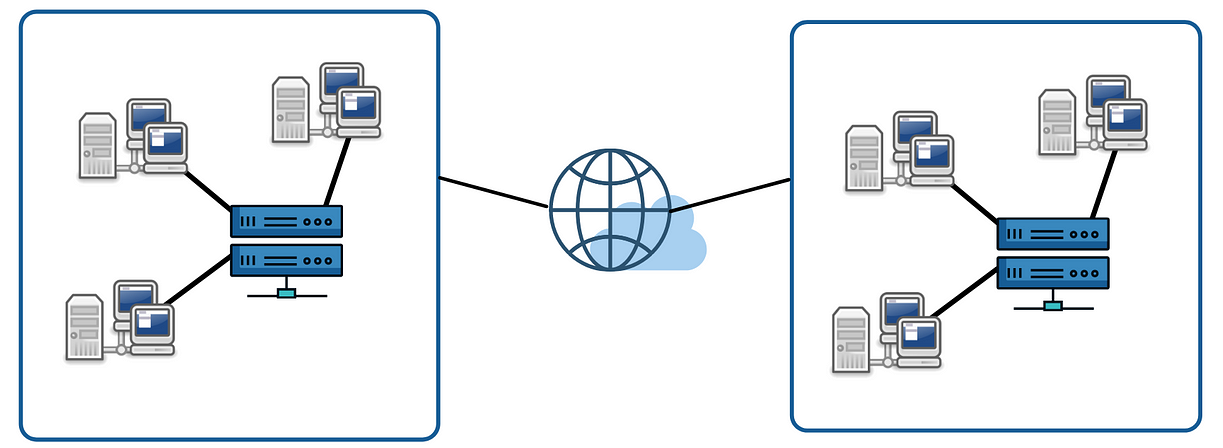
\includegraphics[width=0.8\textwidth]{images/crop.png}
\end{center}
\end{frame}


\begin{frame}{Brief introduction to Choreography Automata}

\begin{itemize}
    \item Chorer: prototype for a static analyzer that extract Choreography 
    Automata from Erlang source code
    \bigskip
    \item Choreography: a formal abstract model for distributed systems
    \bigskip
    \item Choreography Automata: a graphical way of expressing Choreography,
    through LTS
\end{itemize}
\end{frame}

\begin{frame}[fragile]{Case study - Dining philosophers}
Erlang pseudocode:
\begin{lstlisting}
    philosopher(Fork1, Fork2) ->
        send req to Fork1,
        receive ack from Fork1,
        send req to Fork2,
        receive ack from Fork2,
        eat(),
        send release to Fork1,
        send release to Fork2,
        philosopher(Fork1, Fork2).

    fork() ->
        receive req from Phil,
        send ack to Phil,
        receive release from Phil,
        fork().
\end{lstlisting}
\end{frame}


\begin{frame}{Global view example}
\textbf{World} point of view of the communication system

\bigskip

\begin{figure}[t]
\centering
% \makebox[\textwidth][c]{
\resizebox{0.9\textwidth}{!}{%
    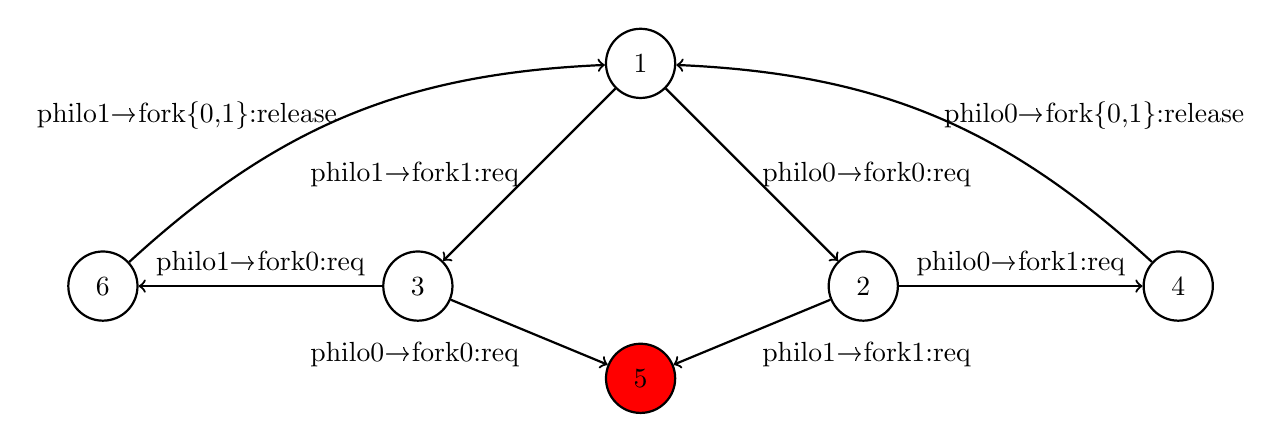
\begin{tikzpicture}[node distance={40mm}, thick, main/.style = {draw, circle}] 
        \node[state] (n_1) {1};
        \node[state] (n_2) [below right of=n_1] {2};
        \node[state] (n_3) [below left of=n_1] {3};
        \node[state] (n_4) [right of=n_2] {4};
        \node[state] (n_5) [below of=n_1, fill=red] {5};
        \node[state] (n_6) [left of=n_3] {6};
        
        \draw[->] (n_1) -- node[midway, right, pos=0.5] {philo0→fork0:req} (n_2);
        \draw[->] (n_1) -- node[midway, left, pos=0.5] {philo1→fork1:req} (n_3);
        \draw[->] (n_2) -- node[midway, below right, pos=0.5] {philo1→fork1:req} (n_5);
        \draw[->] (n_3) -- node[midway, below left, pos=0.5] {philo0→fork0:req} (n_5);
        \draw[->] (n_2) -- node[midway, above, pos=0.5] {philo0→fork1:req} (n_4);
        \draw[->] (n_4) to[bend right=20] node[midway, right, pos=0.5] {philo0→fork\{0,1\}:release} (n_1);
        \draw[->] (n_3) -- node[midway, above, pos=0.5] {philo1→fork0:req} (n_6);
        \draw[->] (n_6) to[bend left=20] node[midway, left, pos=0.5] {philo1→fork\{0,1\}:release} (n_1);
    \end{tikzpicture}
    }
% }%
\caption{Global view of the dining philosophers example.}
\label{graph:philoglobal}
\end{figure}
\end{frame}



\begin{frame}{Local view example}
% mettere in piccolo gv in alto a destra
The point of view of a \textbf{single} actor

\bigskip

\begin{figure}[t]
\centering
% \makebox[\textwidth][c]{
\resizebox{0.8\textwidth}{!}{%
    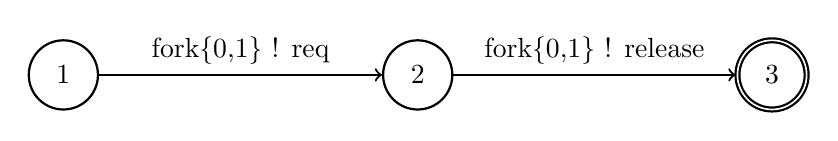
\begin{tikzpicture}[node distance={45mm}, thick, main/.style = {draw, circle}] 
        \node[state] (n_1) {1};
        \node[state] (n_2) [right of=n_1] {2};
        \node[state,accepting] (n_3) [right of=n_2] {3};
        
        \draw[->] (n_1) -- node[midway, above, pos=0.5] {fork\{0,1\} ! req} (n_2);
        \draw[->] (n_2) -- node[midway, above, pos=0.5] {fork\{0,1\} ! release} (n_3);
    \end{tikzpicture}
    }
% }%
\caption{Local view of a philosopher.}
\label{graph:philolocal}
\end{figure}

\begin{figure}[t]
\centering
% \makebox[\textwidth][c]{
\resizebox{0.8\textwidth}{!}{%
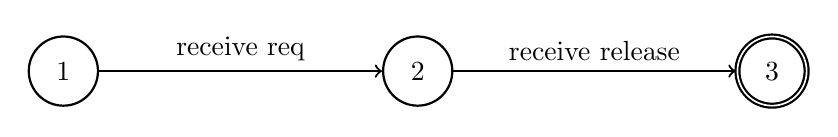
\begin{tikzpicture}[node distance={45mm}, thick, main/.style = {draw, circle}] 
    \node[state] (n_1) {1};
    \node[state] (n_2) [right of=n_1] {2};
    \node[state,accepting] (n_3) [right of=n_2] {3};
    
    \draw[->] (n_1) -- node[midway, above, pos=0.5] {receive req} (n_2);
    \draw[->] (n_2) -- node[midway, above, pos=0.5] {receive release} (n_3);
\end{tikzpicture}
}
% }%
\caption{Local view of a fork.}
\label{graph:forklocal}
\end{figure}
\end{frame}

\begin{frame}{Requirements and challenges}
Requirements:
\begin{itemize}
    \item Automatic \textbf{bottom-up}, \textbf{over-approximated} approach
    \item Always capture the good behaviors, and highlight possible misbehavior
    \item Applicable to mainstream languages
\end{itemize}
\bigskip
Challenges:
\begin{itemize}
    \item Undecidability
    \item Huge descriptions
\end{itemize}
\end{frame}

\section{Chorer}
\begin{frame}{Chorer}
Proof of Concept for a static analyzer
developed as part of a Bachelor’s thesis at the University of Bologna.
Old state:
\bigskip
\begin{itemize}
    \item Few working examples and no case study
    \bigskip
    \item Some important feature missing
    \bigskip
    \item Very difficult to use and understand
    \bigskip
    \item No focus on formalization
\end{itemize}
\end{frame}

\section{Contributions}
\begin{frame}{Contributions}
\begin{itemize}
    \item Formalization journey began (attributed grammar)
    \bigskip
    \item Lots of improvements on the codebase (feature, bug, misc)
    \bigskip
    \item Benchmarks suite improved and case studies created 
\end{itemize}
\end{frame}

\begin{frame}{Attributed grammar}
\begin{itemize}
    \item Formal grammar enriched with attributes assigned to symbols 
    that define how these attributes are computed.
    \bigskip
    \item Used in compilers and parsers design
    \bigskip
    \item Begin a formalization and refactoring process for localviews. 
\end{itemize}
\end{frame}

\begin{frame}[fragile]{Attributed grammar - Example}
% aggiungi slide su storia del tool e focus sugli attributi
$expr \to expr'\ \ !\ \ expr''$
\begin{center}
    \begin{verbatim}
    expr.nodes = expr'.nodes U expr''.nodes U new1 U new2
    expr.edges = expr'.edges U expr''.edges
        U link(expr'.last, expr''.first)
        U link(expr''.last, new1)
        U link(new1, new2, expr'.ret_var 
            + " ! " 
            + expr''.ret_var)
    expr.first = expr'.first
    expr.last = new2
    expr.context = expr'.context U expr''.context
    expr.ret_var = expr''.ret_var
\end{verbatim}
\end{center}
\end{frame}


\begin{frame}{Improvements}
Feature:
\begin{itemize}
    \item Value passing in functions (localview)
    \bigskip
    \item ANY data overapproximation added (globalview)
    \bigskip
    \item Improvements on CLI argument parsing, error and warning report
    \bigskip
    \item Benchmark suite and testing enhanced 
    \bigskip
    \item Some important bugs fixed
\end{itemize}
\end{frame}

% scrivere che sono stati fatti da me
% mettere sample della tabella con casi più interessanti

\begin{frame}{Benchmarks - Empirical data}
\begin{itemize}
    \item Examples made by myself
    \item Show some empirical data about the output produced
    \item Algorithm $O(n!)$ but in practice very efficient 
\end{itemize}

\begin{table}[!ht]
\centering
\begin{tabular}{|c|c|c|c|c|c|c|c|}
\hline
Example & Tot LV & GV Nodes & GV Edges & Warns & Errors & Time \\ 
\hline
async & 3 & 7 & 6 & 0 & 0 & 0.194s \\ 
dining & 3 & 45 & 72 & 0 & 2 & 0.232s \\ 
account & 3 & 28 & 39 & 0 & 2 & 0.211s \\ 
if-cases & 4 & 148 & 210 & 185 & 30 & 0.525s \\ 
foo6 & 5 & 9 & 9 & 15 & 2 & 0.190s \\ 
foo7 & 3 & 149 & 229 & 0 & 6 & 0.513s \\ 
foo8 & 5 & 561 & 560 & 0 & 191 & 3.590s \\ 
\hline
\end{tabular}
\caption{Global view empirical data}
\label{tab:gvbench}
\end{table}
\end{frame}

\begin{frame}{Benchmarks - Correctness}
Set ground for a precision benchmark:

\begin{table}[!ht]
\centering
\begin{tabular}{|c|c|}
\hline
Example & Check \\ 
\hline
unknown & False \\ 
async & True \\ 
ticktackloop & True \\ 
ticktackstop & False \\ 
customer & False \\ 
\hline
\end{tabular}
\caption{Global view correctness data}
\label{tab:corrbench}
\end{table}
\end{frame}


\section{Conclusion}
\begin{frame}{Conclusion}
Key contributions:
\bigskip
\begin{itemize}
    \item Study of the requirements and of the challenges
    \bigskip
    \item Several improvements to the codebase and test suite
    \bigskip
    \item Set groundwork for a formalization process and refactoring
\end{itemize}

\end{frame}


\begin{frame}{Future works}
\begin{itemize}
    \item Continue the formalization and refactoring process
    \bigskip
    \item Extend correctness benchmarks
    \bigskip
    \item Continue feature and bug fix process
\end{itemize}
\end{frame}


\begin{frame}{}
\centering
Thank you for your attention!
\end{frame}


\end{document}